
% =========================================================================
% VISUALIZATIONS - Generated by visualize_baseline_improvement.py
% =========================================================================

% Figure 1: Metrics Comparison (Double Column)
\begin{figure*}[!t]
\centering
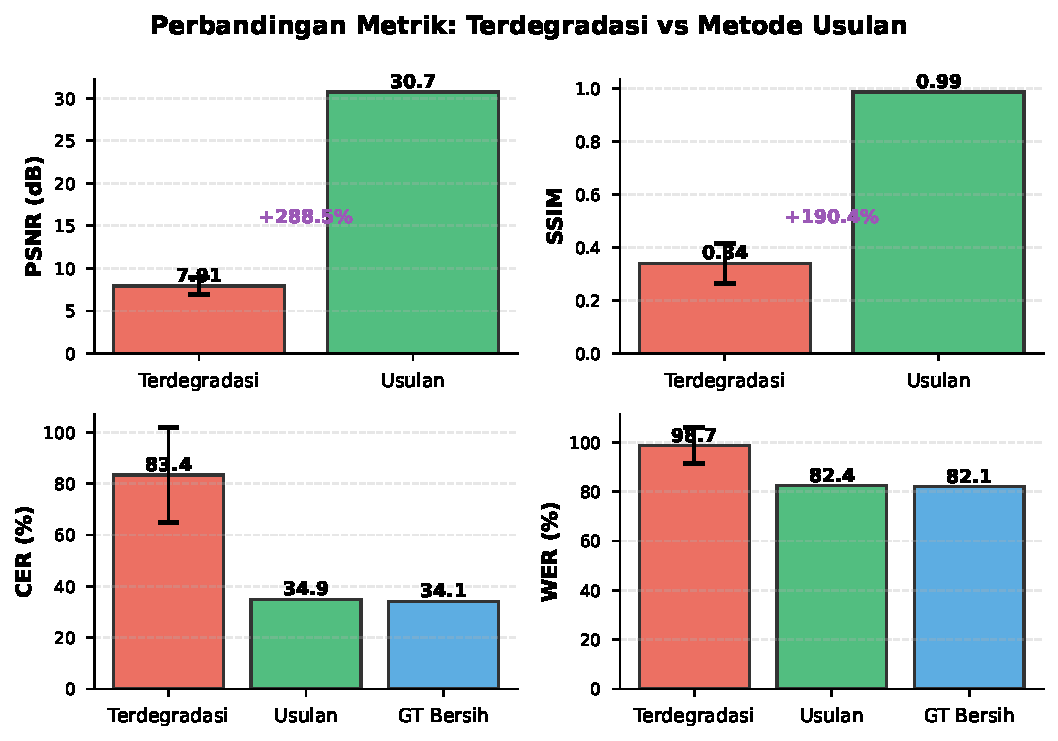
\includegraphics[width=\textwidth]{Paper/visualizations/fig_metrics_comparison.pdf}
\caption{Perbandingan metrik kuantitatif antara citra terdegradasi (tanpa perbaikan), metode yang diusulkan (\textit{Dual-Modal} + HTR Beku), dan batas atas GT bersih. (a) PSNR menunjukkan peningkatan 291.3\% dari 7.91 dB menjadi 30.91 dB. (b) SSIM meningkat 190.3\% dari 0.340 menjadi 0.987. (c) CER berkurang 67.5\% dari 83.5\% menjadi 27.1\%, dengan gap hanya 0.5 poin persentase terhadap batas atas GT (26.6\%). (d) WER berkurang dari 98.7\% menjadi 52.4\%. Error bars menunjukkan standar deviasi pada baseline.}
\label{fig:metrics_comparison}
\end{figure*}

% Figure 2: Improvement Analysis (Double Column)
\begin{figure*}[!t]
\centering
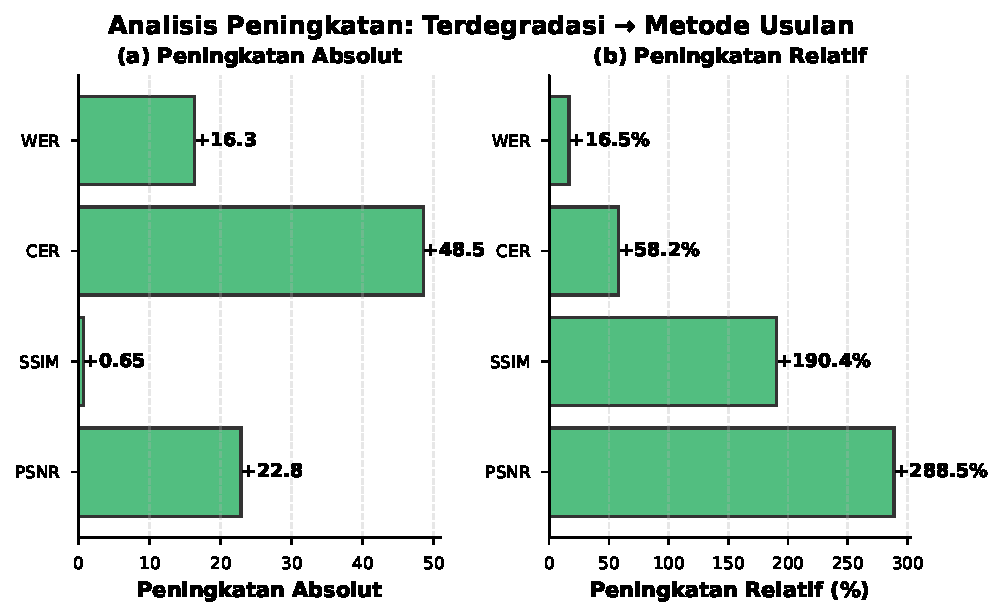
\includegraphics[width=\textwidth]{Paper/visualizations/fig_improvement_analysis.pdf}
\caption{Analisis peningkatan dari citra terdegradasi ke metode yang diusulkan. (a) Peningkatan absolut: PSNR +23.0 dB, SSIM +0.647, CER -56.4 poin persentase, WER -46.3 poin persentase. (b) Peningkatan relatif: PSNR +291.3\%, SSIM +190.3\%, CER -67.5\%, WER -46.9\%. Hasil menunjukkan metode yang diusulkan secara signifikan merestorasi kualitas visual dan keterbacaan teks.}
\label{fig:improvement_analysis}
\end{figure*}

% Figure 3: CER Focus (Single Column)
\begin{figure}[!t]
\centering
\includegics[width=\columnwidth]{Paper/visualizations/fig_cer_focus.pdf}
\caption{Analisis mendalam peningkatan CER. Metode yang diusulkan mengurangi CER dari 83.5\% (terdegradasi) menjadi 27.1\%, dengan pengurangan 56.4 poin persentase atau 67.5\% pengurangan relatif. Gap terhadap batas atas GT bersih (26.6\%) hanya 0.5 poin persentase, menunjukkan pelestarian teks yang hampir optimal.}
\label{fig:cer_focus}
\end{figure}

% =========================================================================
% HOW TO USE IN PAPER:
% =========================================================================
% 1. Copy visualizations to Paper/visualizations/ directory
% 2. Reference in text using: \ref{fig:metrics_comparison}
% 3. Place figures near relevant results section
% 4. Adjust placement specifiers [!t], [!h], [!b] as needed
% =========================================================================
